\documentclass{llncs}

\usepackage{hyperref}

\usepackage[english]{babel}
\usepackage[utf8]{inputenc}
\usepackage[T1]{fontenc}

\usepackage{amsmath}  % Maths
\usepackage{amsfonts} % Maths
\usepackage{amssymb}  % Maths
\usepackage{stmaryrd} % Maths (crochets doubles)

\usepackage{url}     % Mise en forme + liens pour URLs
\usepackage{array}   % Tableaux évolués

\usepackage{comment}


\usepackage{prettyref}
\newrefformat{def}{Def.~\ref{#1}}
\newrefformat{fig}{Fig.~\ref{#1}}
\newrefformat{pro}{Property~\ref{#1}}
\newrefformat{pps}{Proposition~\ref{#1}}
\newrefformat{lem}{Lemma~\ref{#1}}
\newrefformat{thm}{Theorem~\ref{#1}}
\newrefformat{sec}{Sect.~\ref{#1}}
\newrefformat{ssec}{Subsect.~\ref{#1}}
\newrefformat{suppl}{Appendix~\ref{#1}}
\newrefformat{eq}{Eq.~\eqref{#1}}
\def\pref{\prettyref}

\spnewtheorem*{example*}{Example}{\itshape}{}

\usepackage{tikz}
\newdimen\pgfex
\newdimen\pgfem
\usetikzlibrary{arrows,shapes,shadows,scopes}
\usetikzlibrary{positioning}
\usetikzlibrary{matrix}
\usetikzlibrary{decorations.text}
\usetikzlibrary{decorations.pathmorphing}

% Macros relatives à la traduction de PH avec arcs neutralisants vers PH à k-priorités fixes

% Macros générales
\def\Pint{\textsc{PINT}}

% Notations générales pour PH
\newcommand{\PH}{\mathcal{PH}}
\newcommand{\PHs}{\Sigma}
\newcommand{\PHl}{L}
%\newcommand{\PHp}{\mathcal{P}}
\newcommand{\PHp}{\textcolor{red}{\mathcal{P}}}
\newcommand{\PHproc}{\mathcal{P}}
\newcommand{\PHa}{\PHh}
\newcommand{\PHh}{\mathcal{H}}
\newcommand{\PHn}{\mathcal{N}}

\newcommand{\PHhitter}{\mathsf{hitter}}
\newcommand{\PHtarget}{\mathsf{target}}
\newcommand{\PHbounce}{\mathsf{bounce}}
\newcommand{\PHsort}{\Sigma}

\def\f#1{\mathsf{#1}}
\def\focals{\f{focals}}
\def\play{\cdot}
\def\configs#1{\mathbb C_{#1\rightarrow a}}

%\newcommand{\PHfrappeR}{\textcolor{red}{\rightarrow}}
%\newcommand{\PHmonte}{\textcolor{red}{\Rsh}}

\newcommand{\PHfrappeA}{\rightarrow}
\newcommand{\PHfrappeB}{\Rsh}
%\newcommand{\PHfrappe}[3]{\mbox{$#1\PHfrappeA#2\PHfrappeB#3$}}
%\newcommand{\PHfrappebond}[2]{\mbox{$#1\PHfrappeB#2$}}
\newcommand{\PHfrappe}[3]{#1\PHfrappeA#2\PHfrappeB#3}
\newcommand{\PHfrappebond}[2]{#1\PHfrappeB#2}
\newcommand{\PHobjectif}[2]{\mbox{$#1\PHfrappeB^*\!#2$}}
\newcommand{\PHconcat}{::}
\newcommand{\PHneutralise}{\rtimes}

\def\PHget#1#2{{#1[#2]}}
%\newcommand{\PHchange}[2]{#1\langle #2 \rangle}
\newcommand{\PHchange}[2]{(#1 \Lleftarrow #2)}
\newcommand{\PHarcn}[2]{\mbox{$#1\PHneutralise#2$}}
\newcommand{\PHjoue}{\cdot}

\newcommand{\PHetat}[1]{\mbox{$\langle #1 \rangle$}}


% Notations spécifiques à ce papier
\newcommand{\PHdirectpredec}[1]{\PHs^{-1}(#1)}
\newcommand{\PHpredec}[1]{\f{pred}(#1)}
\newcommand{\PHpredecgene}[1]{\f{reg}({#1})}
\newcommand{\PHpredeccs}[1]{\PHpredec{#1} \setminus \Gamma}

\newcommand{\PHincl}[2]{#1 :: #2}

\def\ctx{\varsigma}
\def\ctxOverride{\Cap}
\def\state#1{\langle #1 \rangle}

% Notations spécifiques aux graphes d'états
%\newcommand{\PHge}{\textcolor{red}{\mathcal{GE}}}
%\newcommand{\PHt}{\mathcal{T}}
%\newcommand{\GE}{\mathcal{GE}}
%\newcommand{\GEt}{\mathcal{T}}
%\newcommand{\GEl}{\PHl}
%\newcommand{\GEa}{\PHa}
%\newcommand{\GEva}[3]{#1 \stackrel{#2}{\longrightarrow} #3}
%\newcommand{\GEval}[3]{#1 \stackrel{#2}{\Longrightarrow} #3}
%\newcommand{\GEget}[2]{\PHget{#1}{#2}}


\def\DEF{\stackrel{\Delta}=}
\def\EQDEF{\stackrel{\Delta}\Leftrightarrow}

\def\intervalless{<_{[]}}


\usepackage{ifthen}
\usepackage{tikz}
\usetikzlibrary{arrows,shapes}

\definecolor{lightgray}{rgb}{0.8,0.8,0.8}
\definecolor{lightgrey}{rgb}{0.8,0.8,0.8}

\tikzstyle{boxed ph}=[]
\tikzstyle{sort}=[fill=lightgray,rounded corners]
\tikzstyle{process}=[circle,draw,minimum size=15pt,fill=white,
font=\footnotesize,inner sep=1pt]
\tikzstyle{black process}=[process, fill=black,text=white, font=\bfseries]
\tikzstyle{gray process}=[process, draw=black, fill=lightgray]
\tikzstyle{current process}=[process, draw=black, fill=lightgray]
\tikzstyle{process box}=[white,draw=black,rounded corners]
\tikzstyle{tick label}=[font=\footnotesize]
\tikzstyle{tick}=[black,-]%,densely dotted]
\tikzstyle{hit}=[->,>=angle 45]
\tikzstyle{selfhit}=[min distance=30pt,curve to]
\tikzstyle{bounce}=[densely dotted,->,>=latex]
\tikzstyle{hl}=[font=\bfseries,very thick]
\tikzstyle{hl2}=[hl]
\tikzstyle{nohl}=[font=\normalfont,thin]

\newcommand{\currentScope}{}
\newcommand{\currentSort}{}
\newcommand{\currentSortLabel}{}
\newcommand{\currentAlign}{}
\newcommand{\currentSize}{}

\newcounter{la}
\newcommand{\TSetSortLabel}[2]{
  \expandafter\repcommand\expandafter{\csname TUserSort@#1\endcsname}{#2}
}
\newcommand{\TSort}[4]{
  \renewcommand{\currentScope}{#1}
  \renewcommand{\currentSort}{#2}
  \renewcommand{\currentSize}{#3}
  \renewcommand{\currentAlign}{#4}
  \ifcsname TUserSort@\currentSort\endcsname
    \renewcommand{\currentSortLabel}{\csname TUserSort@\currentSort\endcsname}
  \else
    \renewcommand{\currentSortLabel}{\currentSort}
  \fi
  \begin{scope}[shift={\currentScope}]
  \ifthenelse{\equal{\currentAlign}{l}}{
    \filldraw[process box] (-0.5,-0.5) rectangle (0.5,\currentSize-0.5);
    \node[sort] at (-0.2,\currentSize-0.4) {\currentSortLabel};
   }{\ifthenelse{\equal{\currentAlign}{r}}{
     \filldraw[process box] (-0.5,-0.5) rectangle (0.5,\currentSize-0.5);
     \node[sort] at (0.2,\currentSize-0.4) {\currentSortLabel};
   }{
    \filldraw[process box] (-0.5,-0.5) rectangle (\currentSize-0.5,0.5);
    \ifthenelse{\equal{\currentAlign}{t}}{
      \node[sort,anchor=east] at (-0.3,0.2) {\currentSortLabel};
    }{
      \node[sort] at (-0.6,-0.2) {\currentSortLabel};
    }
   }}
  \setcounter{la}{\currentSize}
  \addtocounter{la}{-1}
  \foreach \i in {0,...,\value{la}} {
    \TProc{\i}
  }
  \end{scope}
}

\newcommand{\TTickProc}[2]{ % pos, label
  \ifthenelse{\equal{\currentAlign}{l}}{
    \draw[tick] (-0.6,#1) -- (-0.4,#1);
    \node[tick label, anchor=east] at (-0.55,#1) {#2};
   }{\ifthenelse{\equal{\currentAlign}{r}}{
    \draw[tick] (0.6,#1) -- (0.4,#1);
    \node[tick label, anchor=west] at (0.55,#1) {#2};
   }{
    \ifthenelse{\equal{\currentAlign}{t}}{
      \draw[tick] (#1,0.6) -- (#1,0.4);
      \node[tick label, anchor=south] at (#1,0.55) {#2};
    }{
      \draw[tick] (#1,-0.6) -- (#1,-0.4);
      \node[tick label, anchor=north] at (#1,-0.55) {#2};
    }
   }}
}
\newcommand{\TSetTick}[3]{
  \expandafter\repcommand\expandafter{\csname TUserTick@#1_#2\endcsname}{#3}
}

\newcommand{\myProc}[3]{
  \ifcsname TUserTick@\currentSort_#1\endcsname
    \TTickProc{#1}{\csname TUserTick@\currentSort_#1\endcsname}
  \else
    \TTickProc{#1}{#1}
  \fi
  \ifthenelse{\equal{\currentAlign}{l}\or\equal{\currentAlign}{r}}{
    \node[#2] (\currentSort_#1) at (0,#1) {#3};
  }{
    \node[#2] (\currentSort_#1) at (#1,0) {#3};
  }
}
\newcommand{\TSetProcStyle}[2]{
  \expandafter\repcommand\expandafter{\csname TUserProcStyle@#1\endcsname}{#2}
}
\newcommand{\TProc}[1]{
  \ifcsname TUserProcStyle@\currentSort_#1\endcsname
    \myProc{#1}{\csname TUserProcStyle@\currentSort_#1\endcsname}{}
  \else
    \myProc{#1}{process}{}
  \fi
}

\newcommand{\repcommand}[2]{
  \providecommand{#1}{#2}
  \renewcommand{#1}{#2}
}
\newcommand{\THit}[5]{
  \path[hit] (#1) edge[#2] (#3#4);
  \expandafter\repcommand\expandafter{\csname TBounce@#3@#5\endcsname}{#4}
}
\newcommand{\TBounce}[4]{
  (#1\csname TBounce@#1@#3\endcsname) edge[#2] (#3#4)
}

\newcommand{\TState}[1]{
  \foreach \proc in {#1} {
    \node[current process] (\proc) at (\proc.center) {};
  }
}

% Macros spécifiques au Modèle de Thomas / aux RRB

% Notations pour le modèle de Thomas (depuis thèse)
\newcommand{\GRN}{\mathcal{GRN}}
\newcommand{\IG}{\mathcal{G}}
%\def\IG{\mathrm{IG}}
\newcommand{\GRNreg}[1]{\Gamma^{-1}(#1)}
\newcommand{\GRNres}[2]{\mathsf{Res}_{#1}(#2)}
\newcommand{\GRNallres}[1]{\mathsf{Res}_{#1}}
\newcommand{\GRNget}[2]{\PHget{#1}{#2}}
\newcommand{\GRNetat}[1]{\PHetat{#1}}

\def\levels{\mathsf{levels}}
\def\levelsA#1#2{\levels_+(#1\rightarrow #2)}
\def\levelsI#1#2{\levels_-(#1\rightarrow #2)}
%\newcommand{\PHres}{\mathsf{Res}}

\newcommand{\Kinconnu}{\emptyset}
\newcommand{\RRGva}[3]{#1 \stackrel{#2}{\longrightarrow} #3}
\newcommand{\RRGgi}{\mathcal{G}}
\newcommand{\RRGreg}[1]{\RRGgi_{#1}}



%\definecolor{darkred}{rgb}{0.5,0,0}
%\definecolor{lightred}{rgb}{1,0.8,0.8}
%\definecolor{lightgreen}{rgb}{0.7,1,0.7}
\definecolor{darkgreen}{rgb}{0,0.5,0}
%\definecolor{darkyellow}{rgb}{0.5,0.5,0}
%\definecolor{lightyellow}{rgb}{1,1,0.6}
%\definecolor{darkcyan}{rgb}{0,0.6,0.6}
%\definecolor{darkorange}{rgb}{0.8,0.2,0}

%\definecolor{notsodarkgreen}{rgb}{0,0.7,0}

%\definecolor{coloract}{rgb}{0,1,0}
%\definecolor{colorinh}{rgb}{1,0,0}
\colorlet{coloract}{darkgreen}
\colorlet{colorinh}{red}
%\colorlet{coloractgray}{lightgreen}
%\colorlet{colorinhgray}{lightred}
%\colorlet{colorinf}{darkgray}
%\colorlet{coloractgray}{lightgreen}
%\colorlet{colorinhgray}{lightred}

%\colorlet{colorgray}{lightgray}


\tikzstyle{grn}=[every node/.style={circle,draw=black,outer sep=2pt,minimum
                size=15pt,text=black}, node distance=1.5cm]
\tikzstyle{act}=[->,draw=black,thick,color=black]
\tikzstyle{inh}=[>=|,-|,draw=black,thick, text=black,label]
%\tikzstyle{inh}=[>=|,-|,draw=colorinh,thick, text=black,label]
%\tikzstyle{act}=[->,>=triangle 60,draw=coloract,thick,color=coloract]
%\tikzstyle{inhgray}=[>=|,-|,draw=colorinhgray,thick, text=black,label]
%\tikzstyle{actgray}=[->,>=triangle 60,draw=coloractgray,thick,color=coloractgray]
\tikzstyle{inf}=[->,draw=colorinf,thick,color=colorinf]
%\tikzstyle{elabel}=[fill=none, above=-1pt, sloped,text=black, minimum size=10pt, outer sep=0, font=\scriptsize,draw=none]
\tikzstyle{elabel}=[fill=none,text=black, above=-2pt,%sloped,
minimum size=10pt, outer sep=0, font=\scriptsize, draw=none]
%\tikzstyle{elabel}=[]
\tikzstyle{sg}=[every node/.style={outer sep=2pt,minimum
                size=15pt,text=black}, node distance=2cm]



% Commandes À FAIRE
\usepackage{color} % Couleurs du texte
%\newcommand{\afaire}[1]{\textcolor{red}{[À FAIRE~: #1]}}
%\newcommand{\resume}[1]{\textcolor{blue}{#1}}
%\newcommand{\todo}[1]{\textcolor{darkgreen}{[#1]}}


% Id est
\newcommand{\ie}{\textit{i.e.} }

% Césures
\hyphenation{pa-ra-me-tri-za-tion}
\hyphenation{pa-ra-me-tri-za-tions}

\title{Concretizing the Process Hitting into Biological Regulatory Networks}

%\author{Maxime Folschette\inst{1,2,}\thanks{This work has been partially supported by the Fondation Centrale Initiatives.}, Lo\"ic Paulev\'e\inst{3}, Katsumi Inoue\inst{2}, Morgan Magnin\inst{1}, Olivier Roux\inst{1}}
\author{Maxime Folschette\inst{1,2}, Lo\"ic Paulev\'e\inst{3}, Katsumi Inoue\inst{2}, Morgan Magnin\inst{1}, Olivier Roux\inst{1}}

\institute{
LUNAM Universit\'e, \'Ecole Centrale de Nantes, IRCCyN UMR CNRS 6597\\
(Institut de Recherche en Communications et Cybern\'etique de Nantes)\\
1 rue de la No\"e - B.P. 92101 - 44321 Nantes Cedex 3, France.\\
\email{Maxime.Folschette@irccyn.ec-nantes.fr}
\and
National Institute of Informatics,\\
2-1-2, Hitotsubashi, Chiyoda-ku, Tokyo 101-8430, Japan.
\and
LIX, \'Ecole Polytechnique, 91128 Palaiseau Cedex, France.
}


\begin{document}

\maketitle

\begin{abstract}
\parindent 0.5cm
The Process Hitting (PH) is a recently introduced framework to model concurrent processes.
Its major originality lies in a specific restriction on the causality of actions, which
makes the formal analysis of very large systems tractable.
PH is suitable to model Biological Regulatory Networks (BRNs) with complete or partial
knowledge of cooperations between regulators by defining the most permissive dynamics
with respect to these constraints.

On the other hand, the qualitative modeling of BRNs has been widely addressed using Ren\'e Thomas'
formalism, leading to numerous theoretical work and practical tools to understand emerging behaviors.

Given a PH model of a BRN, we first tackle the inference of the underlying Interaction Graph
between components.
Then the inference of corresponding Thomas' models is provided using Answer Set Programming,
which allows notably an efficient enumeration of (possibly numerous) compatible parametrizations.

In addition to giving a formal link between different approaches for qualitative BRNs modeling, 
this work emphasizes the ability of PH to deal with large BRNs with incomplete knowledge on
cooperations, where Thomas' approach fails because of the combinatorics of parameters.
\end{abstract}



\section{Introduction}
As regulatory phenomena play a crucial role in biological systems, they need to be studied accurately.
Biological Regulatory Networks (BRNs) consist in sets of either positive or negative mutual effects between the components.
Besides continuous models of physicists, often designed through systems of ordinary
differential equations, a discrete modeling approach was initiated by René Thomas in 1973
\cite{Thomas73} allowing the representation of the different levels of a component, such as concentration or expression levels, as integer values.
%Qualitative state graphs may be derived from which we are able to formally find out all the possible behaviors.
Nevertheless, these dynamics can be precisely established only with regard to some kind of ``focal points'', related to as Thomas' parameters, indicating the evolutionary tendency of each component.

Thomas' modeling (\pref{sec:frameworks}) has motivated numerous works around the link between the influences
%(summarized in the Interaction Graph)
and the possible dynamics (e.g., \cite{RiCo07}), % RRT08
model reduction (e.g., \cite{Naldi09}), %formal checking of dynamics (e.g., \cite{Richard06,Naldi07}), 
or the incorporation of time (e.g., \cite{Siebert06}) % Ahmad08
%and probability (e.g., \cite{Twardziok10-CMSB}) dimensions,
to name but a few.
Other approaches related to our work, which rely on on temporal logic~\cite{Khalis09} and constraint programming~\cite{20646302,DBLP:conf/ipcat/CorblinFTCT12},
aim at determining models consistent with partial data on the regulatory structure and dynamics.
%Our work is also related to the approach of \cite{Khalis09} which relies on temporal logic, and \cite{20646302,DBLP:conf/ipcat/CorblinFTCT12} which uses constraint programming.
%Both aim at determining a class of models which are consistent with available partial data on the regulatory structure and dynamical properties.
While the formal checking of dynamical properties is often limited to small networks because of the
state graph explosion, the main drawback of this framework is the difficulty to specify Thomas'
parameters, especially for large networks.
In our approach, we intend to focus on the Thomas' parameters inference and we claim we are able to deal with networks containing up to 40 components.

In order to address the formal checking of dynamical properties within very large BRNs, we recently
introduced in \cite{PMR10-TCSB} a new formalism, named the \emph{``Process Hitting''} (PH), to model
concurrent systems having components with a few qualitative levels (\pref{sec:frameworks}).
%A PH describes, in an atomic manner, the possible evolution of the level of a component triggered by at most one other component.
Its particular structure makes the formal analysis of BRNs with hundreds components tractable \cite{PMR12-MSCS}.
PH is also suitable to model BRNs with different levels of abstraction in the specification of
associated influences between components by capturing the most general dynamics.

In \cite{FPIMR12-CMSB}, we firstly show (\pref{sec:infer-IG}) that starting from one PH model, it is possible to find back the underlying IG.
We perform an exhaustive search for the possible interactions on one component from all the
others, consistently with the knowledge of the dynamics expressed in PH.
The second phase of our work (\pref{sec:infer-K}) concerns the Thomas' parameters inference.
It consists in abducting the nesting set (possibly large) of parameters which necessarily
lead to the satisfaction of the known cooperating constraints.
%Abduction finally allows to enumerate a family of compatible BRNs whose
The resulting dynamics are ensured to respect the PH dynamics, \ie no spurious transitions are
made possible.

%The first benefit of this work is that such an approach
The first benefit of our approach is that it makes possible the construction refining of BRNs with a partial and progressively brought knowledge in PH, while being able to export such models in the Thomas' framework.
Our second contribution is to enhance the knowledge of the formal links between both modelings.
As BRNs are not limited to boolean values, the whole method can be applied to multi-valued models;
furthermore, the method can be applied to large BRNs.

\begin{comment}
\paragraph{Outline.}
\pref{sec:frameworks} recalls the PH and Thomas frameworks;
\pref{sec:infer-IG} defines the IG inference from PH;
\pref{sec:infer-K} details the enumeration of Thomas parametrizations compatible with a PH;
%and discuss its implementation in ASP.
\pref{sec:examples} gives some information about the implementation of the method.
%illustrates the applicability of our method on simple examples
%and large biological models.
\end{comment}


\section{Frameworks}\label{sec:frameworks}
\subsection{The Process Hitting framework}
\label{ssec:PH}

A PH (\pref{def:PH}) gathers a finite number of concurrent \emph{processes}
grouped into a finite set of \emph{sorts}.
A process belongs to a unique sort and is noted $a_i$ where $a$ is the
sort and $i$ the identifier of the process within the sort $a$.
At any time, one and only one process of each sort is present; a state of the PH thus corresponds to the set of such processes.
 
The concurrent interactions between processes are defined by a set of
\emph{actions}.
Actions describe the replacement of a process by another of the same sort
conditioned by the presence of at most one other process in the current
state of the PH.
An action is denoted by $\PHfrappe{a_i}{b_j}{b_k}$ where $a_i,b_j,b_k$ are processes
of sorts $a$ and $b$.
An action $h=\PHfrappe{a_i}{b_j}{b_k}$ is read as ``$a_i$ \emph{hits} $b_j$ to
make it bounce to $b_k$'', and
$a_i,b_j,b_k$ are called respectively \emph{hitter}, \emph{target} and
\emph{bounce} of the action, and can be referred to as
$\PHhitter(h), \PHtarget(h), \PHbounce(h)$, respectively.

\begin{definition}[Process Hitting]\label{def:PH}
A \emph{Process Hitting} is a triple $(\PHs,\PHl,\PHa)$:
\begin{itemize}
\item $\PHs \DEF \{a,b,\dots\}$ is the finite set of \emph{sorts};
\item $\PHl \DEF \prod_{a\in\PHs} \PHl_a$ is the set of states with $\PHl_a = \{a_0,\dots,a_{l_a}\}$
the finite set of \emph{processes} of sort $a\in\Sigma$ and $l_a$ a positive integer with
	$a\neq b\Rightarrow \forall(a_i,b_j)\in\PHl_a\times\PHl_b,a_i\neq b_j$;
\item $\PHa \DEF \{ \PHfrappe{a_i}{b_j}{b_k}, \dots \mid
					(a,b)\in\PHs^2 \wedge (a_i,b_j,b_k)\in \PHl_a\times\PHl_b\times\PHl_b$ \\
	\hspace*{2cm} $\wedge b_j\neq b_k \wedge a=b\Rightarrow a_i=b_j\}$
			is the finite set of \emph{actions}.
\end{itemize}
$\PHproc$ denotes the set of all processes ($\PHproc \DEF \{ a_i\mid a\in\PHs \wedge a_i\in\PHl_a\}$).
\end{definition}

\noindent
The sort of a process $a_i$ is referred to as $\PHsort(a_i)=a$ and the set of
sorts present in an action $h\in\PHa$ as 
$\PHsort(h) = \{\PHsort(\PHhitter(h)),\PHsort(\PHtarget(h))\}$.
Given a state $s\in \PHl$, the process of sort $a\in\PHs$ present in $s$ is
denoted by $\PHget{s}{a}$, that is the $a$-coordinate of the state $s$.
If $a_i\in \PHl_a$, we define the notation $a_i\in s \EQDEF \PHget{s}{a}=a_i$.

An action $h=\PHfrappe{a_i}{b_j}{b_k} \in\PHa$ is \emph{playable} in $s\in L$
if and only if $\PHget{s}{a}=a_i$ and $\PHget{s}{b}=b_j$.
In such a case, $(s\play h)$ stands for the state resulting from the play of
the action $h$ in $s$, that is 
$\PHget{(s\play h)}{b} = b_k$ and 
$\forall c\in\PHs, c\neq b, \PHget{(s\play h)}{c} = \PHget{s}{c}$.
For the sake of clarity, $((s\play h)\play h')$, $h'\in\PHa$ is abbreviated as
$(s\play h\play h')$.

\paragraph{Modeling cooperation.}
As described in \cite{PMR10-TCSB}, cooperation between processes to make another process bounce can be
expressed in PH by building a \emph{cooperative sort}.
\pref{fig:runningPH} shows an example of cooperation between processes $b_1$ and $c_1$ to
make $a_1$ bounce to $a_2$:
a cooperative sort $bc$ is defined with 4 processes (one for each sub-state of the presence of
processes $b_1$ and $c_1$), and the process $bc_{11}$ hits $a_1$ instead of the processes
$b_1$ and $c_1$ independently.
We note that cooperative sorts are standard PH sorts and do not involve any
special treatment regarding the semantics of related actions.

While the construction of cooperation in PH allows to encode any boolean functions
between cooperating processes, it is worth noticing they introduce a temporal
shift in their application.
This allows the existence of interleaving of actions leading to a cooperative sort representing a
past sub-state of the presence of the cooperative processes.
The resulting behavior is then an over-approximation of the realization of an instantaneous
cooperation.

\begin{example*}
\pref{fig:runningPH} represents a PH $(\PHs,\PHl,\PHa)$ with especially:
$\PHs = \{a,b,c,bc\}$,
$\PHl_a = \{a_0,a_1,a_2\}$,
$\PHl_b = \{b_0, b_1\}$,
$\PHl_c = \{c_0, c_1\}$ and
$\PHl_{bc} = \{bc_{00}, bc_{01}, bc_{10}, bc_{11}\}$.
%Furthermore, the action $h=\PHfrappe{b_1}{a_1}{a_2}$ is playable in the state
%$s = \state{b_1,a_1,c_0}$; and $s\play h=\state{b_1,a_2,c_0}$.

\begin{comment}
\begin{figure}[t]
\centering
\scalebox{1.3}{
\begin{tikzpicture}
\TSort{(0,0)}{a}{3}{r}
\TSort{(-3,0.5)}{b}{2}{l}
\TSort{(3,0.5)}{c}{2}{r}

\THit{b_1}{very thick}{a_0}{.west}{a_1}
\THit{b_1}{very thick}{a_1}{.north west}{a_2}
\THit{b_0}{}{a_2}{.west}{a_1}
\THit{b_0}{}{a_1}{.west}{a_0}

\path[bounce, bend left=60]
\TBounce{a_1}{very thick}{a_2}{.south}
\TBounce{a_0}{very thick}{a_1}{.south}
;
\path[bounce, bend right=60]
\TBounce{a_2}{}{a_1}{.north}
\TBounce{a_1}{}{a_0}{.north}
;

\THit{c_1}{very thick}{a_0}{.east}{a_1}
\THit{c_1}{very thick}{a_1}{.north east}{a_2}
\THit{c_0}{}{a_2}{.east}{a_1}
\THit{c_0}{}{a_1}{.east}{a_0}

\path[bounce, bend right=60]
\TBounce{a_1}{very thick}{a_2}{.south east}
\TBounce{a_0}{very thick}{a_1}{.south east}
;
\path[bounce, bend left=60]
\TBounce{a_2}{}{a_1}{.north}
\TBounce{a_1}{}{a_0}{.north east}
;

\THit{a_2}{bend right}{b_1}{.north east}{b_0}
\path[bounce, bend left=80]
\TBounce{b_1}{out=100,in=140}{b_0}{.north}
;

\end{tikzpicture}
}
\caption{\label{fig:runningPH-1}
A Process Hitting (PH) example.
Sorts are represented by labeled boxes, and processes by circles (ticks are
the identifiers of the processes within the sort, for instance, $a_0$ is the
process ticked $0$ in the box $a$).
An action (for instance $\PHfrappe{b_1}{a_1}{a_2}$) is represented by a pair of
directed arcs, having the hit part ($b_1$ to $a_1$) in plain line and the bounce
part ($a_1$ to $a_2$) in dotted line.
Actions involving $b_1$ or $c_1$ are in thick lines.
%The current state is represented by the grayed processes:
%$\state{a_0,b_1,c_0,d_0}$.
}
\end{figure}

\end{comment}

This PH example actually models a BRN where the component $a$ has three qualitative
levels and components $b$ and $c$ are boolean.
In this BRN, $a$ inhibits $b$ (when its level is at $2$) while $b$ and $c$ activate $a$ both independently (with direct actions such as
$\PHfrappe{b_0}{a_2}{a_1}$) or through a cooperation (with action defined from the cooperative sort $bc$, such as
$\PHfrappe{bc_{11}}{a_1}{a_2}$).
Hence, this PH expresses a BRN where $a$ requires both $b$ and $c$ active to reach its
highest level, and $a$ does not become inactive unless both $b$ and $c$ are inactive.
\end{example*}

\subsection{Thomas' modeling}
Thomas' formalism, here inspired by \cite{Richard06,BernotSemBRN}, lies on two complementary descriptions of the system.
First, the \emph{Interaction Graph} (IG) models the structure of the system by defining the components' mutual influences.
Its nodes represent components, while its edges labeled with a threshold stand for either positive or negative interactions (\pref{def:ig});
$l_a$ denotes the maximum level of a component $a$.

\begin{definition}[Interaction Graph]
\label{def:ig}
An \emph{Interaction Graph} (IG) is a triple $(\Gamma, E_+, E_-)$ where $\Gamma$ is a finite number of \emph{components},
and $E_+$ (resp. $E_-$) $\subset \{a \xrightarrow{t} b \mid a, b \in \Gamma \wedge t \in [1; l_a]\}$
is the set of positive (resp. negative) \emph{regulations} between two nodes, labeled with a \emph{threshold}.

A regulation from $a$ to $b$ is uniquely referenced:
if $a \xrightarrow{t} b \in E_+$ (resp. $E_-$),
then $\nexists a \xrightarrow{t'} b \in E_+ \text{ (resp. $E_-$)}, t' \neq t$
and $\nexists a \xrightarrow{t'} b \in E_-\text{ (resp. $E_+$)}, t' \in \mathbb{N}$.
\end{definition}

\noindent
For an interaction of the IG to take place, the expression level of its head component has to be higher than its threshold; otherwise, the opposite influence is expressed.
For any component $a \in \Gamma$, $\GRNreg{a} = \{ b\in\Gamma\mid \exists b\xrightarrow t a\in E_+\cup E_- \}$
is the set of its regulators.
A \emph{state} $s$ of an IG $(\Gamma, E_+, E_-)$ is an element in $\prod_{a \in \Gamma} [0;l_a]$
and $\GRNget{s}{a}$ refers to the level of component $a$ in $s$.

Then, the specificity of Thomas' approach lies in the use of discrete \emph{parameters} to represent focal level intervals (\pref{def:param}).
While the use of intervals as parameters does not add expressivity in Boolean networks, it allows to specify a larger range of dynamics in the general case (w.r.t. a fixed IG).
%Indeed, if a parameter is an interval of three values, it is impossible to split the three cases with the boolean definition of resources.

\begin{definition}[Discrete parameter $K_{x,A,B}$ and Parametrization $K$]\label{def:param}
Let $x \in \Gamma$ be a given component and $A$ (resp. $B$) $\subset \GRNreg{x}$ a set of its \emph{activators} (resp. \emph{inhibitors}),
such that $A \cup B = \GRNreg{x}$ and $A \cap B = \emptyset$.
The discrete \emph{parameter} $K_{x,A,B} = [i; j]$ is a non-empty interval so that $0 \leq i \leq j \leq l_x$.
With regard to the dynamics, $x$ will tend towards $K_{x,A,B}$ in the states where its activators (resp. inhibitors) are the regulators in set $A$ (resp. $B$).
The complete map $K = (K_{x,A,B})_{x,A,B}$ of discrete parameters for an IG is called a \emph{parametrization} of this IG.
\end{definition}

At last, dynamics are defined in BRN in an unitary and asynchronous way:
from a given state $s$, a transition to another state $s'$ is possible provided that only one component $a$ will evolve of exactly one level towards $K_{a,A,B}$, where $A$ (resp. $B$) is the set of activators (resp. inhibitors) of $a$ in $s$.

\begin{example*}
\pref{fig:runningBRN}(left) represents an Interaction Graph $(\Gamma,E_+,E_-)$ with
$\Gamma = \{a, b, c\}$,
$E_+ = \{b \xrightarrow{1} a, c \xrightarrow{1} a\}$ and
$E_- = \{a \xrightarrow{2} b\}$;
hence $\GRNreg{a} = \{b, c\}$.
\pref{fig:runningBRN}(right) gives a possible parametrization on this IG.
In this BRN, the following transitions are possible:
$\GRNetat{a_0, b_1, c_1} \rightarrow \GRNetat{a_1, b_1, c_1} \rightarrow \GRNetat{a_2, b_1, c_1} \rightarrow
\GRNetat{a_2, b_0, c_1} \rightarrow \GRNetat{a_1, b_0, c_1}$,
where $a_i$ is the component $a$ at level $i$.
\end{example*}

\begin{figure}[t]
\begin{minipage}{0.4\linewidth}
\centering
\scalebox{1.2}{
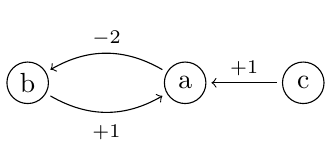
\begin{tikzpicture}[grn]
\path[use as bounding box] (0,-0.7) rectangle (3.5,0.7);
\node[inner sep=0] (a) at (2,0) {a};
\node[inner sep=0] (b) at (0,0) {b};
\node[inner sep=0] (c) at (3.5,0) {c};
%\path
%  node[elabel, below=-1em of a] {$0..2$}
%  node[elabel, below=-1em of b] {$0..1$}
%  node[elabel, below=-1em of c] {$0..1$};
\path[->]
  (b) edge[bend right] node[elabel, below=-3pt] {$+1$} (a)
  (c) edge node[elabel, above=-5pt] {$+1$} (a)
  (a) edge[bend right] node[elabel, above=-5pt] {$-2$} (b);
\end{tikzpicture}
}
\end{minipage}
\begin{minipage}{0.6\linewidth}
\centering
\begin{align*}
K_{a,\{b,c\},\emptyset} &= [2 ; 2] & K_{b,\{a\},\emptyset} &= [0 ; 1] \\
K_{a,\{b\},\{c\}} &= [1 ; 1] & K_{b,\emptyset,\{a\}} &= [0 ; 0] \\
K_{a,\{c\},\{b\}} &= [1 ; 1] &&\\
K_{a,\emptyset,\{b,c\}} &= [0 ; 0] & K_{c,\emptyset,\emptyset} &= [0 ; 1]
\end{align*}
\end{minipage}
\caption{\label{fig:runningBRN}
(left)
IG example.
Regulations are represented by the edges labeled with their sign and threshold.
For instance, the edge from $b$ to $a$ is labeled $+1$, which stands for: $b \xrightarrow{1} a \in
E_+$.
(right)
Example parametrization of the left IG.
}
\end{figure}


\section{Interaction Graph Inference}\label{sec:infer-IG}

In order to infer a complete BRN, one has to find the Interaction Graph (IG) first, as some
constraints on the parametrization rely on it.
Inferring the IG is an abstraction step which consists in determining the global influence of
components on each of its successors.

This section first introduces the notion of focal processes within a PH
(\pref{ssec:focal}) which is used to characterize well-formed PH for IG inference
in \pref{ssec:wf}, and as well used by the parametrization inference presented in \pref{sec:infer-K}.
Finally, the rules for inferring the interactions between components from a PH are
described in \pref{ssec:infer-IG}.
We consider hereafter a global PH $(\PHs,\PHl,\PHa)$ on which the IG inference is to be
performed.

\subsection{Focal Processes}\label{ssec:focal}

Many of the inferences defined in the rest of this paper rely on the knowledge of \emph{focal
processes} w.r.t. a given context (a set of processes that are potentially present).
When such a context applies, we expect to (always) reach one focal process in a bounded number of
actions.

For $S_a\subseteq L_a$ and a context (set of processes) $\ctx$, let us define as $\PHa(S_a,\ctx)$
the set of actions on the sort $a$ having their hitter in $\ctx$ and target in $S_a$
(\pref{eq:PHa-ctx});
and the digraph $(V, E)$ where arcs are the bounces within the sort $a$ triggered by actions
in $\PHa(S_a,\ctx)$ (\pref{eq:bounce-graph}).
$\focals(a,S_a,\ctx)$ denotes the set of focal processes of sort $a$ in the scope of
$\PHa(S_a,\ctx)$ (\pref{def:focals}).
\begin{align}
\PHa(S_a,\ctx) & \DEF \{ \PHfrappe{b_i}{a_j}{a_k}\in\PHa \mid b_i\in\ctx \wedge a_j\in S_a \}
\label{eq:PHa-ctx}
\\
\begin{split}
E  & \DEF \{(a_j,a_k)\in (S_a \times \PHl_a) \mid 
			\exists\PHfrappe{b_i}{a_j}{a_k}\in \PHa(S_a,\ctx) \}
\\
V & \DEF S_a \cup \{ a_k\in L_a\mid \exists (a_j,a_k)\in E\}
\end{split}
\label{eq:bounce-graph}
\end{align}

\begin{definition}[$\focals(a,S_a,\ctx)$]\label{def:focals}
The set of processes that are focal for processes in $S_a$ in the scope of $\PHa(S_a,\ctx)$
are given by:
%$\focals(a,S_a,\ctx)$ is the set of focal processes of sort $a$ in the context $\ctx$:
\[
\focals(a,S_a,\ctx) \DEF
\begin{cases}
\{ a_i \in V \mid \nexists (a_i,a_j)\in E\} & \text{if the digraph $(V,E)$ is acyclic},\\
\emptyset & \text{otherwise.}\\
\end{cases}
\]
\end{definition}

We note $\PHl(\ctx)$ the set of states $s\in L$ such that $\forall a\in\PHsort(\ctx), \PHget{s}{a}\in\ctx$,
where $\PHsort(\ctx)$ is the set of sorts with processes in $\ctx$.
We say a sequence of actions $h^1,\dots,h^n$ is \emph{bounce-wise} if and only if
$\forall m\in[1;n-1], \PHbounce(h^m)=\PHtarget(h^{m+1})$.
From \pref{def:focals}, it derives that:
\begin{enumerate}
\item if $\focals(a,S_a,\ctx)=\emptyset$, there exists a 
state $s\in \PHl(\ctx\cup S_a)$ such that $\forall n\in\mathbb N$ there
exists a bounce-wise sequence of actions $h^1,\dots,h^{n+1}$ in $\PHa(S_a,\ctx)$ 
with $\PHtarget(h^1)\in s$.
\item if $\focals(a,S_a,\ctx)\neq\emptyset$, for all
state $s\in \PHl(\ctx\cup S_a)$,
for any bounce-wise sequence of actions $h^1,\dots,h^n$ in $\PHa(S_a,\ctx)$ where $\PHtarget(h^1)\in
s$,
either
 $\PHbounce(h^n) \in \focals(a,S_a,\ctx)$,
or
$\exists h^{n+1}\in \PHa(a,\ctx)$ such that $\PHbounce(h^n) = \PHtarget(h^{n+1})$.
Moreover $n\leq|\PHa(S_a,\ctx)|$ (i.e. no cycle of actions possible).
\end{enumerate}

It is worth noticing that those bounce-wise sequences of actions may not be successively playable in
a state $s\in L(\ctx\cup S_a)$.
Indeed, nothing impose that the hitters of actions are present in $s$.
In the general case, the playability of those bounce-wise sequences, referred to as \emph{focals
reachability} may be hard to prove.
However, in the scope of this paper, the particular contexts used with $\focals$ ensure this property.
Notably, the rest of this section uses only \emph{strict} contexts (\pref{def:strict-ctx}) which
allow at most one hitter per sort in the bounce-wise sequences (and thus are present in $s$).

\begin{comment}
\begin{property}[$\focals$ reachability]\label{pro:focals-reach}
$\focals(a,S_a,\ctx)$ is reachable if and only if 
$\forall s\in L(\ctx\cup S_a)$,
if $\exists h\in \PHa(S_a,\ctx)$ with $\PHtarget(h)\in s$,
there exists a (possibly empty) sequence of actions
$h^1,\dots,h^n \in \PHa(\ctx\cup S_a)$
	such that $h^1,\dots,h^n,h$ are successively playable in $s$;
where $\PHa(\ctx) \DEF \{ \PHfrappe{b_i}{c_j}{c_k}\in\PHa \mid c\neq a \wedge
			b\in \PHsort(\ctx) \Rightarrow b_i\in \ctx \wedge c\in\PHsort(\ctx) \Rightarrow
			c_i\in\ctx \}$.
\end{property}
\end{comment}

\begin{definition}[Strict context for $S_a$]\label{def:strict-ctx}
A context (set of processes) $\ctx$ is strict for $S_a\subseteq L_a$ if and only if
$\{b_i,b_j\} \subset \ctx \wedge b\neq a \Rightarrow i=j$.
\end{definition}

In other words, assuming focals reachability, if $\focals(a,S_a,\ctx)$ is empty, there exists a
sequence of actions that may be played an unbound number of times (cycle);
if it is non-empty, it is ensured that any state in $\PHl(\ctx\cup S_a)$ converges, in a bounded
number of steps, either to a process in $S_a$ that is not hit by processes in $\ctx$, or to a process in
$L_a\setminus S_a$.

\begin{example*}
In the PH of \pref{fig:runningPH-1}, we obtain:
\begin{align*}
\focals(a,L_a,\{b_0,c_0\}) &= \{ a_0 \}
&
\focals(a,L_a,\{b_1,c_1\}) &= \{ a_2 \}
\\
\focals(a,L_a,\{b_1,c_0\}) &= \emptyset
&
\focals(a,\{a_1\},\{b_1,c_0\}) &= \{ a_0, a_2 \}
\end{align*}
\end{example*}

\subsection{Well-formed Process Hitting for Interaction Graph Inference}\label{ssec:wf}

The inference of an IG from a PH assumes that the PH defines two types of sorts:
the sorts corresponding to BRN components, and the cooperative sorts.
This leads to the characterization of a \emph{well-formed} PH for IG inference.

The identification of sorts modeling components relies on the observation that their processes
represent (ordered) qualitative levels.
Hence an action on such a sort cannot make it bounce to a process at a distance more than one.
The set of sorts satisfying such a condition is referred to as $\Gamma$
(\pref{eq:PH-components}).
Therefore, in the rest of this paper, $\Gamma$ denotes the set of components of the BRN to infer.

\begin{equation}
\Gamma \DEF \{a \in \PHs \mid \nexists \PHfrappe{b_i}{a_j}{a_k} \in \PHa, |j - k| > 1\} \\
\label{eq:PH-components}
\end{equation}

Any sort that does not act as a component should then be treated as a cooperative sort.
As explained in \pref{ssec:PH}, the role of a cooperative sort $\upsilon$ is to compute the current
state of set of cooperating processes.
Hence, for each sub-state $\sigma$ formed by the sorts hitting $\upsilon$, $\upsilon$ should
converge to a focal process.
This is expressed by \pref{pro:wf-cooperative-sort}, where
the set of sorts having an action on a given sort $a$ is given by 
$\PHdirectpredec{a}$ (\pref{eq:ph_direct_predec})
and $\PHproc(\sigma)$ is the set of processes that compose the sub-state $\sigma$.

\begin{equation}
\forall a \in \PHs, \PHdirectpredec{a} \DEF \{b \in \PHs \mid \exists \PHfrappe{b_i}{a_j}{a_k}\in\PHa \}
\label{eq:ph_direct_predec}
\end{equation}

\begin{property}[Well-formed cooperative sort]\label{pro:wf-cooperative-sort}
A sort $\upsilon\in\PHs$ is a well-formed cooperative sort if and only if
each configuration $\sigma$ of its predecessors leads $\upsilon$ to a unique focal process,
denoted by $\upsilon(\sigma)$:
\[
\forall \sigma \in {\textstyle\prod_{
a\in\PHdirectpredec{\upsilon} \wedge a\neq \upsilon}}
\PHl_{a},
\focals(\upsilon,\PHl_\upsilon,\PHproc(\sigma)\cup \PHl_\upsilon) = \{ \upsilon(\sigma) \}\]
\end{property}

Such a property allows a large variety of definitions of a cooperative sort, but
for the sake of simplicity, does not allow the existence of multiple focal processes.
While this may be easily extended to (the condition becomes 
$\focals(\upsilon,\PHl_\upsilon, \PHproc(\sigma)\cup \PHl_\upsilon)\neq\emptyset$), it makes some
hereafter equations a bit more complex to read as they should handle a set of focal processes instead
of a unique focal process.


Finally, \pref{pro:wf-ph} sums up the conditions for a Process Hitting to be suitable for IG
inference.
In addition of having either component sorts or well-formed cooperative sorts, we also require that
there is no cycle between cooperative sorts, and that
sorts being never hit (\ie{} serving as an invariant environment) are components.

\begin{property}[Well-formed Process Hitting for IG inference]\label{pro:wf-ph}
A PH is well-formed for IG inference if and only if the following conditions are verified:
\begin{itemize}
\item 
each sort $a\in\PHs$ either belongs to $\Gamma$, or is a well-formed cooperative sort;
\item 
there is no cycle between cooperative sorts
(the digraph $(\Sigma,\{(a,b)\in(\Sigma\times\Sigma)\mid \exists \PHfrappe{a_i}{b_j}{b_k}\in\PHa
\wedge a\neq b\wedge \{a,b\}\cap\Gamma=\emptyset \})$ is
acyclic);
\item 
sorts having no action hitting them belong to $\Gamma$
($\{ a \in \Sigma\mid \nexists \PHfrappe{b_i}{a_j}{a_k}\in\PHa\} \subset \Gamma$).
\end{itemize}
\end{property}

\begin{example*}
In the PH of \pref{fig:runningPH-2}, $bc$ is a well-formed cooperative sort as defined in \pref{pro:wf-cooperative-sort}, because:
\begin{align*}
\focals(bc, \PHl_{bc}, \{b_0, c_0\} \cup \PHl_{bc}) = \{bc_{00}\} && \focals(bc, \PHl_{bc}, \{b_0, c_1\} \cup \PHl_{bc}) = \{bc_{01}\} \\
\focals(bc, \PHl_{bc}, \{b_1, c_0\} \cup \PHl_{bc}) = \{bc_{10}\} && \focals(bc, \PHl_{bc}, \{b_1, c_1\} \cup \PHl_{bc}) = \{bc_{11}\}
\end{align*}
Hence, both \pref{fig:runningPH-1} and \pref{fig:runningPH-2} are well-formed PH for IG inference
with $\Gamma = \{a,b,c\}$.
\end{example*}


\subsection{Interaction Inference}\label{ssec:infer-IG}

At this point we can divide the set of sorts $\PHs$ into components ($\Gamma$, see \pref{eq:PH-components}) and cooperative sorts
($\PHs \setminus \Gamma$) that will not appear in the IG. 
We define in \pref{eq:ph_predec} the set of predecessors of a sort $a$, that is, the sorts influencing $a$
by considering direct actions and possible intermediate cooperative sorts.
The predecessors of $a$ that are components are the regulators of $a$, denoted $\PHpredecgene{a}$
(\pref{eq:regulators}).
\begin{align}
\begin{split}
\forall a \in \PHs, \PHpredec{a} &\DEF \{b \in \PHs \mid \exists n \in \mathbb{N}^*, \exists
(c^k)_{k \in [0;n]} \in \PHs^{n+1}, \\
                                   & \quad \quad c^0 = b \wedge c^n = a \\
                                   & \quad \quad \wedge \forall k \in \llbracket 0 ; n-1 \rrbracket,
								   c^k \in \PHdirectpredec{c^{k+1}} \cap (\PHs\setminus\Gamma)\}
\end{split}
\label{eq:ph_predec}
\\
\forall a\in \PHs, \PHpredecgene{a} & \DEF \PHpredec{a} \cap \Gamma
\label{eq:regulators}
\end{align}

Given a set $g$ of components and a configuration (\ie a sub-state) $\sigma$, $\ctx_g(\sigma)$
refers to the set of processes hitting $a$ regulated by any sort in $g$ (\pref{eq:ctx-sigma}).
If $g=\{b\}$, we simple note $\ctx_b(\sigma)$.
This set is composed of the active processes of sorts in $g$, and the focal process (assumed
unique) of the cooperative sorts $\upsilon$ hitting $a$ that have a predecessor in $g$.
The evaluation of the focal process of $\upsilon$ in context $\sigma$, denoted $\upsilon(\sigma)$,
relies on \pref{pro:wf-cooperative-sort}, which gives its value when all the direct predecessors of
$\upsilon$ are defined in $\sigma$.
When a predecessor $\upsilon'$ is not in $\sigma$, we extend the evaluation by recursively computing
the focal value of $\upsilon'$ is $\sigma$, as stated in \pref{eq:cooperative-eval}.
Because there is no cycle between cooperative sorts, this recursive evaluation of $\upsilon(\sigma)$
always terminates.
\begin{align}
\forall g\subset \Gamma,
	\ctx_g(\sigma) & \DEF \{ \sigma[b] \mid b\in g \} \cup \{ \upsilon(\sigma) \mid
\upsilon\in\PHdirectpredec{a} \setminus \Gamma \wedge g\cap \PHpredecgene{\upsilon} \neq \emptyset \}
\label{eq:ctx-sigma}
\\
\upsilon(\sigma) & \DEF
\upsilon(\sigma \uplus \state{\upsilon'(\sigma) \mid 
	\upsilon'\in\PHdirectpredec{\upsilon} \wedge
	\upsilon'\in\PHs\setminus\Gamma })
\label{eq:cooperative-eval}
\end{align}

We aim at inferring that $b$ activates (inhibits) $a$ if there exists a configuration where increasing
the level of $b$ makes possible the increase (decrease) of the level of $a$.
This is analogous to standard IG inferences from discrete maps \cite{RiCo07}.

This reasoning can be straightforwardly applied to a PH when inferring the influence of $b$ on $a$
when $b\neq a$ (\pref{eq:edges-inference-b}).
Let us define $\gamma(b\rightarrow a)$ as the set of components cooperating with $b$ to hit $a$,
including $b$ and $a$ (\pref{eq:cooperating-with-b}).
Given a configuration $\sigma\in\prod_{c\in\gamma(b\rightarrow a)} L_c$, 
$\focals(a,\{a_i\},\ctx_b(\sigma))$ gives the bounces that a given process $a_i$ can make in the
context $\ctx_b(\sigma)$.
We note $\sigma\{b_i\}$ the configuration $\sigma$ where the process of sort $b$ has been replaced
by $b_i$.
If there exists $b_i,b_{i+1}\in L_b$ such that one bounce in 
$\focals(a, \{\sigma[a]\}, \ctx_b(\sigma\{b_i\}))$
has a lower (resp. higher) level that one bounce in
$\focals(a, \{\sigma[a]\}, \ctx_b(\sigma\{b_{i+1}\}))$, then
$b$ as positive (resp. negative) influence on $a$ with a maximum threshold $l=i+1$.
\begin{equation}
\gamma(b\rightarrow a)  \DEF \{ a, b \} \cup \{ c \in \Gamma \mid 
			\exists \upsilon\in\PHs\setminus\Gamma,
				\upsilon\in\PHpredec{a} \wedge \{b,c\}\subset\PHpredec{\upsilon} \}
\label{eq:cooperating-with-b}
\end{equation}


Then, we infer that $a$ has a self-influence if its current level can have an impact on its own
evolution at a given configuration $\sigma$.
We consider here a configuration $\sigma$ of a group $g$ of sorts having a cooperation on $a$.
This set of sort groups is given by $X(a)$ (\pref{eq:influence-groups}) which returns the set of
connected components (noted $\mathcal C$) of the graph linking two regulators $b,c$ of $a$ if there
is a cooperative sort hitting $a$ regulated by both of them.
Given $a_i,a_{i+1}\in L_a$, we pick $a_j\in\focals(a,\{a_i\},\ctx_g(\sigma\{a_i\}))$ and
$a_k\in\focals(a,\{a_{i+1}\},\ctx_g(\sigma\{a_{i+1}\}))$.
If $k=j+1$, we can not conclude as there is no difference in the evolution of both levels.
If $k\neq j+1$ and $k-j\neq 0$, then $a_i$ and $a_{i+1}$ have divergent evolutions: we infer an
influence of sign of $k-j$ at threshold $i+1$.
We note that some aspects of this inference are arbitrary and may impact the number of parameters to
infer in the next section.
In particular, in some cases, the use of intervals for Thomas' parameters drops the requirement of
inferring a self-activation.
%Future work may propose alternative definitions of self-influences inference in order to range over
%different parametrization configurations.
\begin{equation}
X(a) = \mathcal C\left( (\PHpredecgene{a}, \{ \{b,c\} \mid
				\exists \upsilon\in \PHdirectpredec{a} \setminus \Gamma,
					\{b,c\} \subset \PHpredecgene{\upsilon} \}) \right)
\label{eq:influence-groups}
\end{equation}

\pref{pps:inference-edges} details the inference of all existing influences between components occurring
with a threshold $l$.
These influences are split into positive and negative ones, and represent possible edges in the final IG.
We do not consider the cases where a component has no visible influence on another.
\begin{proposition}[Edges inference]\label{pps:inference-edges}
We define the set of positive (resp. negative) influences $\hat{E}_+$ (resp. $\hat{E}_-$) for any
$a\in\Gamma$ by:
\begin{align}
\begin{split}
\forall b\in\PHpredecgene{a}, b\neq a, \\
b\xrightarrow l a \in \hat{E}_s & \Longleftrightarrow
 \exists \sigma\in\textstyle\prod_{c\in\gamma(b\rightarrow a)} L_c, \exists b_i,b_{i+1}\in \PHl_b,\\
& \qquad\qquad
        \exists a_{j}\in\focals(a, \{\sigma[a]\}, \ctx_b(\sigma\{b_i\})), \\
& \qquad\qquad
        \exists a_{k}\in\focals(a, \{\sigma[a]\}, \ctx_b(\sigma\{b_{i+1}\})), \\
& \qquad\qquad\qquad
                        s = \f{sign}(k - j) \wedge l = i+1
\end{split}
\label{eq:edges-inference-b}
\\
\begin{split}
a \xrightarrow l a \in \hat{E}_s & \Longleftrightarrow
\exists g \in X(a), \sigma \in L_a\times \textstyle\prod_{b\in g} L_b,
			\exists a_i,a_{i+1}\in \PHl_a, \\
& \qquad\qquad
        \exists a_{j}\in\focals(a, \{a_i\}, \ctx_g(\sigma\{a_i\})), \\
& \qquad\qquad
        \exists a_{k}\in\focals(a, \{a_{i+1}\},  \ctx_g(\sigma\{a_{i+1}\})), \\
& \qquad\qquad\quad
			k \neq j+1
				\wedge s = \f{sign}(k - j) \wedge l = i+1
\end{split}
\label{eq:edges-inference-a}
\end{align}
where $s \in \{ +, - \}$, $\bar s = + \EQDEF s = -$, $\bar s = - \EQDEF s = +$,
$\f{sign}(n) = + \EQDEF n > 0$,
$\f{sign}(n) = - \EQDEF n < 0$,
and $\f{sign}(0) \DEF 0$.
\end{proposition}

We are now able to infer the edges of the final IG by considering positive and negative influences
(\pref{pps:inference-IG}).
We infer a positive (resp. negative) edge if there exists a corresponding influence with the same
sign. If an influence is both positive and negative, we infer an unsigned edge. In the end, the
threshold of each edge is the minimum threshold for which the influence has been found. As unsigned
edges represent ambiguous interactions, no threshold is inferred.
\begin{proposition}[Interaction Graph inference]\label{pps:inference-IG}
We infer $\IG = (\Gamma,E_+,E_-,E_\pm)$ from \pref{pps:inference-edges} as follows:
\begin{align*}
E_+ &= \{a \xrightarrow{t} b \mid \nexists a \xrightarrow{t'} b \in \hat{E}_-
  \wedge t = \min \{ l \mid a \xrightarrow{l} b \in \hat{E}_+\}\} \\
E_- &= \{a \xrightarrow{t} b \mid \nexists a \xrightarrow{t'} b \in \hat{E}_+
  \wedge t = \min \{l \mid a \xrightarrow{l} b \in \hat{E}_-\}\} \\
E_\pm &= \{a \rightarrow b \mid \exists a \xrightarrow{t} b \in \hat{E}_+ \wedge \exists a \xrightarrow{t'} b \in \hat{E}_-\} \\
\end{align*}
\end{proposition}


\begin{example*}
The IG inference from the PH of \pref{fig:runningPH-2} gives
$\hat{E}_+ = \{b \xrightarrow{1} a, c \xrightarrow{1} a\}$ and 
$\hat{E}_- = \{a \xrightarrow{2} b\}$, corresponding to the IG of \pref{fig:runningBRN}.
No self-influence are inferred ($X(a) = \{ \{b,c\} \}$, $X(b)=\{ \{a\}\}$, and $X(c)=\emptyset$).
\end{example*}

\section{Parametrization inference}\label{sec:infer-K}

Given the IG inferred from a PH as presented in the previous section, one can find the discrete parameters that model the behavior of the studied PH using the method presented in the following.
As some parameters may remain undetermined, another step allows to enumerate all parametrizations compatible with the inferred parameters.

\subsection{Independent parameters inference}

This subsection presents some results related to the inference of independent discrete parameters from a given PH,
equivalent to those presented in \cite{PMR10-TCSB}.
We suppose in the following that the considered PH is well-formed for parameters inference: its inferred IG does not contain any unsigned edge,
and in each sort, all processes activating (resp inhibiting) another component share the same behavior.
Let $K_{a,A,B}$ be the parameter we want to infer for a given component $a \in \Gamma$
and $A \subset \GRNreg{a}$ (resp. $B \subset \GRNreg{a}$) a set of its activators (resp. inhibitors).
This inference, as for the IG inference, relies on the search of focal processes of the component for the given configuration of its regulators.

For each sort $b \in \GRNreg{a}$, we define a context
that represents the influence of the regulators in the configuration $A,B$ (including the cooperative sorts involved).
The parameter $K_{a,A,B}$ specifies to which values $a$ eventually evolves as long as the context
holds, which is precisely given by the set of focal processes.

\begin{example*}
Applied to the PH in \pref{fig:runningPH}, we obtain, in particular,
$K_{b,\{a\},\emptyset} = [0 ; 1]$,
$K_{a,\{b,c\},\emptyset} = [2 ; 2]$ and
$K_{a,\{b\},\{c\}} = [1;1]$.
\end{example*}

This method sometimes faces cases with opposite effects on a component, leading to either an indeterministic evolution or to oscillations.
Such an indeterminism is not possible in a BRN, and the inference of the targeted parameter is impossible.
In order to avoid such inconclusive cases, one has to ensure that no such behavior is allowed
by either removing undesired actions or using cooperative sorts to prevent opposite influences between regulators.

\subsection{Admissible parametrizations}\label{ssec:admissible-K}

In the following, we try to constrain all parameters that are left undetermined with the method presented in the previous subsection.
We consider that a parameter is valid if any transition it involves in the resulting BRN is allowed by the studied PH by actions that represent this behavior.
We also add some biological constraints on the whole parametrizations, given in \cite{BernotSemBRN}.
These constraints lead to a family of admissible parametrizations which we can enumerate and are ensured to observe a coherent behavior that is included in the original PH.

This approach can be considered as abductive reasoning as some information is added by the enumeration.
If we denote:
\begin{itemize}
  \item $M$ the resulting BRN that observes a behavior included into the one of the original PH,
  \item $B$ the IG and the series of necessary parameters inferred from the original PH,
  \item $H_K$ the hypothesis that we select the complete parametrization $K$
\end{itemize}
The set of parametrizations $K$ that answers our expectations are the ones so that:
\begin{itemize}
  \item $H_K$ is compatible with $B$, that is, all parameters of $K$ are compatible with the inferred parameters in $B$,
  \item $B \wedge H_K \models M$, that is, the parametrization $K$ found from enumeration and the inferred IG represent a BRN observing the behavior included into the behavior of the original PH.
\end{itemize}

Answer Set Programming (ASP) \cite{Baral03} turns out to be effective for the enumerative searches developed in this paper,
as it efficiently tackles with the inherent complexity of the models we use, thus allowing an efficient execution of the formal tools developed.
Furthermore, ASP finds a particularly interesting application in the research of admissible parametrizations regarding the properties presented above, as this enumeration can be naturally formulated with the use of aggregates, and constraints allow to remove all non-admissible models.



\begin{comment}
\subsection{Answer Set Programming implementation concepts}

\newcommand{\ti}[1]{\texttt{\textit{#1}}}
\newcommand{\aspil}[1]{\texttt{#1}}
\newcommand{\asp}[1]{\begin{itemize} \item[] \aspil{#1} \end{itemize}}


All information describing the studied model (PH and inferred IG \& parameters) can be expressed in ASP using facts.
For functional purposes, we assign a unique label to each couple $A,B$ of activators and inhibitors of a given component, which allows to refer to the related parameter (in the following, we note $K^p_{a,A,B}$ the parameter of component $a$ whose regulators $A,B$ are assigned to the label $p$).
Consequently, to express that it exists a parameter of component \ti{a} with the label \ti{p}, we use an atom named \aspil{param\_label} in the following fact:
\asp{param\_label(\ti{a}, \ti{p}).}

Defining a set in ASP is equivalent to defining the rule for belonging to this set. For example, we can define an atom \aspil{param\_act} that describes the set of all active regulators for a parameter of component \ti{a} and label \ti{p} (\ie the set $A$ of a parameter $K^\ti{p}_{\ti{a},A,B}$). For example, describing the activators of $K^\ti{p}_{\ti{a},\{\ti{b},\ti{c}\},\{\ti{d}\}}$ gives:
\asp{param\_act(\ti{a}, \ti{p}, \ti{b}).
\item[] param\_act(\ti{a}, \ti{p}, \ti{c}).}
The absence of such a fact involving \ti{d} with label \ti{p} indicates that \ti{d} is an inhibitor in the configuration of regulators related to this parameter.

Rules allow more detailed declarations than facts as they have a body (right-hand part below) containing constraints and allowing to use variables, while facts only have a head (left-hand part).
For instance, in order to define the set of expression levels of a component, we can declare:
\asp{component\_levels(X, 0..M) :- component(X, M).}
where the \aspil{component(X, M)} atom stands for the existence of a component \aspil{X} with a maximum level \aspil{M}.
Considering this declaration, any possible answer for the atom \aspil{component\_levels} will be found by binding all possible values of its terms with all existing \aspil{component} facts: an answer \aspil{component\_levels(\ti{a}, \ti{k})} will depend on the existence of a term \ti{a}, which is bound with \aspil{X}, and an integer~\ti{k}, constrained by: $0 \leq \ti{k} \leq \aspil{M}$.

Cardinalities are convenient to enumerate all possible parametrizations by creating multiple answer sets.
A cardinality (denoted hereafter with curly brackets) gives any number of possible answers for some atoms between a lower and upper bounds.
For example,
\asp{1 \{ param(X, P, I) : component\_levels(X, I) \} :-
\item[] ~~~~~~param\_label(X, P), not infered\_param(X, P).}
where \aspil{param(X, P, I)} stands for: $\aspil{I} \in K^\aspil{P}_{\aspil{X},A,B}$,
means that any parameter of component \aspil{X} and label \aspil{P} must contain at least one level value (\aspil{I}) in the possible expression levels of \aspil{X}.
Indeed, the lower bound is 1, forcing at least one element in the parameter, but no upper bound is specified, allowing up to any number of answers.
The body (right-hand side) of the rule also checks for the existence of a parameter of \aspil{X} with label \aspil{P}, and constrains that the parametrization inference was not conclusive for the considered parameter (\aspil{not} stands for negation by failure: \aspil{not L} becomes true if \aspil{L} is not true).
Such a constraint gives multiple results as any set of \aspil{param} atoms satisfying the cardinality will lead to a new global set of answers.
In this way, we can enumerate all possible parametrizations which respects the results of parameters
inference, but completely disregarding the notion of admissible parametrizations given in
\pref{ssec:admissible-K}.

We rely on integrity constraints to filter only admissible parametrizations.
An integrity constraint is a rule with no head, that makes an answer set unsatisfiable if its body turns out to be true.
Hence, supposing that:
\begin{itemize}
  \item the \aspil{less\_active(\ti{a}, \ti{p}, \ti{q})} atom means that $K^\ti{p}_{\ti{a},A,B}$ stands for a configuration with less activating regulators than $K^\ti{q}_{\ti{a},A',B'}$ (\ie $A \subset A'$),
  \item the \aspil{param\_inf(\ti{a}, \ti{p}, \ti{q})} atom means: $K^\ti{p}_{\ti{a},A,B} \leq_{[]} K^\ti{q}_{\ti{a},A',B'}$,
\end{itemize}
then the monotonicity assumption can be formulated as the following integrity constraint:
\asp{:- less\_active(X, P, Q), not param\_inf(X, P, Q).}
which removes all parametrization results where parameters $K^\aspil{P}_{\aspil{X},A,B}$ and $K^\aspil{Q}_{\aspil{X},A',B'}$ exist such that $A \subset A'$ and $K^\aspil{Q}_{\aspil{X},A',B'} <_{[]} K^\aspil{P}_{\aspil{X},A,B}$, thus violating the monotonicity assumption.
Of course, other assumptions can be formulated in the same way.

This subsection succinctly described how we write ASP programs to represent a model and solve all steps of Thomas' modeling inference.
It finds a particularly interesting application in the enumeration of parameters: all possible parametrizations are generated in separate answer sets, and integrity constraints are formulated to remove those that do not fit the assumptions of admissible parametrizations,
thus reducing the number of interesting parametrizations to be considered in the end.
\end{comment}

\section{Implementation}\label{sec:examples}

The inference method described in this paper has been implemented as a tool named \texttt{ph2thomas}, as part of
\textsc{Pint}\footnote{Available at \url{http://process.hitting.free.fr}}, which gathers PH related
tools.
Our implementation mainly consists in ASP programs that are solved using Clingo\footnote{Available
at \url{http://potassco.sourceforge.net}}.

In the previous sections and in the appendix, we illustrate our results on toy examples considered as small networks.
%which contains 3 components and is considered as a small network.
But our approach can also successfully handle large PH models of BRNs found in the literature
such as an ERBB receptor-regulated G1/S transition model from \cite{Sahin09} which contains 20
components, and a T-cells receptor model from \cite{Klamt06} which contains 40
components\footnote{Both models are available as examples distributed with \textsc{Pint}.}.
For each model, IG and parameters inferences are performed together in less than a second
on a standard desktop computer.



\begin{comment}
The inference method described in this paper has been implemented as part of
\textsc{Pint}\footnote{Available at \url{http://process.hitting.free.fr}}, which gathers PH related
tools.
Our implementation mainly consists in ASP programs that are solved using Clingo\footnote{Available
at \url{http://potassco.sourceforge.net}}.
The IG and parameters inference can be performed using the command
\texttt{ph2thomas -i model.ph -{}-dot ig.dot}
where \texttt{model.ph} is the PH model in \textsc{Pint} format and \texttt{ig.dot} is an output of the inferred IG in DOT format.
The (possibly partial) inferred parametrization will be returned on the standard output.
The admissible parametrizations enumeration is performed when adding the \texttt{-{}-enumerate}
parameter to the command.

Applied to the example in \pref{fig:runningPH-2} where cooperations have been defined,
our method infers the IG and parametrization given in \pref{fig:runningBRN}.
Regarding the example in \pref{fig:runningPH-1}, the same IG is inferred, as well as for the
parametrization except for the parameters $K_{a,\{b\},\{c\}}$ and $K_{a,\{c\},\{b\}}$ which are
undefined (because of the lack of cooperativity between $b$ and $c$).
In such a case, this partial parametrization allows 36 admissible complete parametrizations, as two
parameters with 3 potential values could not be inferred.
If we constrain these latter parameters so that they contain exactly one element, we obtain only 9
admissible parametrizations.

The current implementation can successfully handle large PH models of BRNs found in the literature
such as an ERBB receptor-regulated G1/S transition model from \cite{Sahin09} which contains 20
components, and a T-cells receptor model from \cite{Klamt06} which contains 40
components\footnote{Both models are available as examples distributed with \textsc{Pint}.}.
For each model, IG and parameters inferences are performed together in less than a second
on a standard desktop computer.
%\footnote{Using a Dell Inspiron 1720 laptop, with an Intel Core 2 Duo CPU T5550 ($2 \times 1.83\text{GHz}$)
%and 3.9 Gib memory, on an Ubuntu 11.10 64-bits OS}
After removing the cooperations from these models (leaving only raw actions), the inferences allow to
determine 40 parameters out of 195 for the 20 components model, and 77 out of 143 for the 40 components model.
As we thus have an order of magnitude of respectively $10^{31}$ and $10^{73}$ admissible parametrizations,
this model would therefore be more efficiently studied as a PH than as a BRN.
We note that the complexity of the method is exponential in the number of regulators of one
component and linear in the number of components.
% We note that despite its smaller size in term of components, the ERBB transmission model takes more time to be computed because the biggest cooperative sorts contain more processes (up to 32 processes) than in the T-cells receptor model (up to 8 processes).
\end{comment}

\section{Conclusion}

This work establishes the abstraction relationship between PH, which is more abstract and allows incomplete knowledge on cooperations, and Thomas' approach for qualitative BRN modeling.
This motivates the concretization of PH models into a set of compatible Thomas' models in order to benefit of the complementary advantages of these two formal frameworks and extract some global information about the influences between components.

As an extension of the presented work, we plan to explore new semantics of BRNs that would be able to tackle with influences currently represented by unsigned edges.

\paragraph{Ack.}
This work was partially supported by the Fondation Centrale Initiatives.


\bibliographystyle{splncs}
\bibliography{biblio}

\appendix
\section*{Contributions}

The division of the effort for this paper is: M. Folschette: 50\% (theory, implementation, redaction); L. Paulev\'e: 30\%
(theory, redaction); K. Inoue, M. Magnin, O. Roux: 20\% (redaction).

\medskip

The individual contributions are the following:

\medskip

\noindent
M. Folschette (PhD student):
\begin{itemize}
  \item Theory:
  \begin{itemize}
    \item Worked on the IG inference
    \item Worked on the parameters enumeration
    \item Worked on the components/cooperative sorts distinction
  \end{itemize}
  \item Implementation: programmed all logic parts (IG inference, parameters inference and parametrization enumeration) and result processing for the \texttt{ph2thomas} tool
  \item Redaction (sections 2, 4 \& 5)
\end{itemize}

\noindent
L. Paulevé:
\begin{itemize}
  \item Theory:
  \begin{itemize}
    \item Worked on the formalism (use of focals)
    \item Worked on the “well-formed” notions
    \item Previous publication about parameters inference
  \end{itemize}
  \item Implementation: integration of \texttt{ph2thomas} into \textsc{Pint}
  \item Redaction (abstract, sections 1, 2, 3 \& 6)
\end{itemize}

\noindent
K. Inoue, M. Magnin \& O. Roux:
\begin{itemize}
  \item Redaction (abstract, sections 1 \& 4)
\end{itemize}


\end{document}
